% Mo Jabeen Template for docs 

\documentclass[11pt]{scrartcl} % Font size

%%%%%%%%%%%%%%%%%%%%%%%%%%%%%%%%%%%%%%%%%
% Wenneker Assignment
% Structure Specification File
% Version 2.0 (12/1/2019)
%
% This template originates from:
% http://www.LaTeXTemplates.com
%
% Authors:
% Vel (vel@LaTeXTemplates.com)
% Frits Wenneker
%
% License:
% CC BY-NC-SA 3.0 (http://creativecommons.org/licenses/by-nc-sa/3.0/)
% 
%%%%%%%%%%%%%%%%%%%%%%%%%%%%%%%%%%%%%%%%%

%----------------------------------------------------------------------------------------
%	PACKAGES AND OTHER DOCUMENT CONFIGURATIONS
%----------------------------------------------------------------------------------------

\usepackage{amsmath, amsfonts, amsthm} % Math packages

\usepackage{listings} % Code listings, with syntax highlighting

\usepackage[english]{babel} % English language hyphenation

\usepackage{graphicx} % Required for inserting images
\graphicspath{{Figures/}{./}} % Specifies where to look for included images (trailing slash required)

\usepackage{booktabs} % Required for better horizontal rules in tables

\numberwithin{equation}{section} % Number equations within sections (i.e. 1.1, 1.2, 2.1, 2.2 instead of 1, 2, 3, 4)
\numberwithin{figure}{section} % Number figures within sections (i.e. 1.1, 1.2, 2.1, 2.2 instead of 1, 2, 3, 4)
\numberwithin{table}{section} % Number tables within sections (i.e. 1.1, 1.2, 2.1, 2.2 instead of 1, 2, 3, 4)

\setlength\parindent{0pt} % Removes all indentation from paragraphs

\usepackage{enumitem} % Required for list customisation
\setlist{noitemsep} % No spacing between list items

%----------------------------------------------------------------------------------------
%	DOCUMENT MARGINS
%----------------------------------------------------------------------------------------

\usepackage{geometry} % Required for adjusting page dimensions and margins

\geometry{
	paper=a4paper, % Paper size, change to letterpaper for US letter size
	top=2.5cm, % Top margin
	bottom=3cm, % Bottom margin
	left=3cm, % Left margin
	right=3cm, % Right margin
	headheight=0.75cm, % Header height
	footskip=1.5cm, % Space from the bottom margin to the baseline of the footer
	headsep=0.75cm, % Space from the top margin to the baseline of the header
	%showframe, % Uncomment to show how the type block is set on the page
}

%----------------------------------------------------------------------------------------
%	FONTS
%----------------------------------------------------------------------------------------

\usepackage[utf8]{inputenc} % Required for inputting international characters
\usepackage[T1]{fontenc} % Use 8-bit encoding

\usepackage{fourier} % Use the Adobe Utopia font for the document

%----------------------------------------------------------------------------------------
%	SECTION TITLES
%----------------------------------------------------------------------------------------

\usepackage{sectsty} % Allows customising section commands

\sectionfont{\vspace{6pt}\centering\normalfont\upshape} % \section{} styling
\subsectionfont{\normalfont\bfseries} % \subsection{} styling
\subsubsectionfont{\normalfont\itshape} % \subsubsection{} styling
\paragraphfont{\normalfont\scshape} % \paragraph{} styling

%----------------------------------------------------------------------------------------
%	HEADERS AND FOOTERS
%----------------------------------------------------------------------------------------

\usepackage{scrlayer-scrpage} % Required for customising headers and footers

\ohead*{} % Right header
\ihead*{} % Left header
\chead*{} % Centre header

\ofoot*{} % Right footer
\ifoot*{} % Left footer
\cfoot*{\pagemark} % Centre footer

\usepackage{array}
\newcolumntype{P}[1]{>{\centering\arraybackslash}p{#1}}
 % Include the file specifying the document structure and custom commands

%----------------------------------------------------------------------------------------
%	TITLE SECTION
%----------------------------------------------------------------------------------------

\title{	
	\normalfont\normalsize
	\vspace{20pt} % Whitespace
	{\huge Intro To Statistical Learning: Notes}\\ % The meh
	\vspace{12pt} % Whitespace
	\rule{\linewidth}{2pt}\\ % Thick bottom horizontal rule
}

\author{\small Mo D Jabeen} % Your name

\date{\normalsize\today} % Today's date (\today) or a custom date

\begin{document}

\maketitle % Print the title

\section{General}

Statsictal is learning is based on making predictions or inferences on data inputs. Via approximating f(x),
where y = f(x) + error.

\subsection{What are the types of statistical problems?}

\begin{itemize}
	\item Regression: Determine outcome variable based on predictors, continous problem ie Range of values 
	\item Classification: Discrete choice of answers (normally qualitative)
	\item Clustering: Determine similar groups of data (no natural output variable)
\end{itemize}

\subsection{Notation}

\begin{equation}
	x_{ij}, i:1,2,\cdots n, j:1,2,\cdots p
\end{equation}
\begin{equation}
	x_{i} = (x{i1},x_{i2},x_{i3} \cdots,x_{ip})
\end{equation}

i is the observation and j is the predictor.

\subsection{What is paramtric and non parametric?}

\textbf{Parametric:} Assume form of the desired function and calculate parameters based on the assumption.\\

\textbf{Non Parametric:} Do not make any explicit assumptions, instead fit function best to the data given.\\

Choosing an non parametric avoids the problem of having a function form very differnt to reality however opens up
the possibility of overfitting (following noise too closely) and needs more data for an accurate form.\\

Furthermore, if the main goal is inference, restrictive (parametric) are much easier to interpret.

\subsection{What is unsupervised learning?}

There is no response/outcome variable, ie clustering.\\

\textbf{Semi supervised learning:} some response variables.

\subsection{What is RSS?}

Resiudal sum of squares is minimised in regression to calculate the parameters.

\begin{equation}
	RSS = (y_1-\beta_0-\beta_1x_1)^2 + \cdots +(y_n-\beta_0-\beta_1x_n)^2
\end{equation}

\section{Quality of fit}

Measure how well the model fits the the true model.

\subsection{How is Mean Squared Error used?}

Regression compares the predicted outcome to the true value and measures the MSE. However many
statistical methods minimise the \textbf{training} MSE, therefore a test MSE should be used!\\

If there is a small training MSE and a large test MSE this can indicate overfitting.

\begin{equation}
	MSE = \frac{1}{n}\sum^n_{i=1}{(y_i-\hat{f}(x_i))^2}
\end{equation}

\subsection{What is Bias Variance Trade off?}

MSE can be deconstructed to give variance of the estimate function, squared bias of the estimate function
and variance of error.

\begin{equation}
	E(y_o - \hat{f}(x_o))^2 = Var(\hat{f}(x_o)) + (Bias(\hat{f}(x_o)))^2 + Var(\epsilon)
\end{equation}

Aim is to minimise variance and bias as error can not be removed.

The rate of change between var and bias determines optimal flexibilty of a model.

\subsubsection{What is variance?}

The change in outcome/model if the data set is changed. Higher flexibilty of model often increases
this.

\subsubsection{What is bias?}

Error from approximations.

\subsection{Error Rate}

Classification accuracy is measured by error rate, the frequency of values that predicted the wrong class. In this
case test error rate is also preffered.

\begin{equation}
	Error\; rate = \frac{1}{n} \sum{I(y_i \neq \hat{y_i})} , I: y_i \neq \hat{y_i} ? 1:0
\end{equation}

\subsection{What is Bayes Classification?}

Choosing the max probablilty an observation is a class will minimise the error rate.

Ie if there are only two classes, choose the class that fits:
\begin{equation}
	P(Y=1|X=x_o) > 0.5
\end{equation}

\subsection{What is Bayes error rate?}

\begin{equation}
	Bayes\; Error\; Rate = 1 - E(maxP(Y=j|X=x_o))
\end{equation}

E is the average for all values of X. ie if the probablilty of a 2 class, setup where one class is 0.7 the error rate
will be 0.3. Not possible to actually use Bayes as the probablilty is unknown, however, this is the gold standard.

\section{Classification}

\subsection{What is K nearest neighbours?}

KNN identifies the K points closest to training point x, shown as \(\eta_o\). The conditional probablilty is then
the fraction of the points in \(\eta_o\) that equal class j.

\begin{equation}
	P(Y=j|X=X_o) = \frac{1}{K}\sum_{i\epsilon \eta_o}{I(y_i=j)}
\end{equation}

Then classify point x as the class with the highest probablilty. K =1 has low bias but high variance.

\subsection{Why logistic regression instead of linear regression?}

To create a regression problem from a classification, you would be forced to create some type of ordering of the qualitative
variables if >2. This ordering may not be true for the data set. However with a binary classification least squares is possible, the
issue is that least squares does not have the required boundaries for a binary decison ie 0-1 so you would create a useless areas.

\subsection{What is logistic regression?}

To bound p(X) between 0 and 1, exponential equation is used:

\begin{equation}
	p(X) = P(Y=1|X)
\end{equation}

\begin{equation}
	p(X) = \frac{e^{\beta_0 + \beta_1X}}{1+e^{\beta_0 + \beta_1X}}
\end{equation}

This will produce an S curve, and if the log is taken shows that 1 unit increase in X gives a change of log odds by 
\( \beta_1\).

\begin{equation}
	log\; odds: ln(\frac{p(X)}{1-p(X)}) = \beta_0 + \beta_1X
\end{equation}

This also shows that if \(\beta_1\) is postive, increasing X will increase p(X), if negative the increasing X will
decrease p(X).

\subsection{How is logistic regression used?}

For binary class scenarios you are trying to maximise the liklehood function to estimate the beta parameters.

Likelhood function:
\begin{equation}
	(\beta_o,\beta_1) = \Pi_{i:Y_i=1}p(x_i) + \Pi_{i:Y_i=0}(1-p(x_i))
\end{equation}

\subsection{What is standard error?}

\begin{equation}
	SE(\alpha^2) = x
	\label{normalSE}
\end{equation}

\ref{normalSE} shows for each sample expect \(\alpha\) to very by x on average.

The below is the standard erorr of the mean ie std/n:

\begin{equation}
	SE(\mu)^2 = \frac{\sigma^2}{n}
\end{equation}

The below is based on how the Betas are calculated (this is for linear regression):

\begin{equation}
	SE(\hat{\beta_0})^2 = \sigma^2(\frac{1}{n} + \frac{\bar{x}^2}{\sum{(x_i-\bar{x})^2}})
\end{equation}

\begin{equation}
	SE(\beta_1)^2 = \frac{\sigma^2}{\sum{(x_i-\bar{x})^2}}
\end{equation}



\subsection{What ways can you validate the parameters?}

Use confidence intervals, z/t tests and hypothesis tests.\\

The null hypothesis is that there is no relationship between predictor and outcome.

\subsection{What are dummy variables?}

If there is qualitative category for the observational data, this can be used a dummy value which is used to represent
the observations. This then requires new parameters to be calculated.\\

I.e. set \(x_i\) as 1 if male, 0 if female. If more than one category use multiple pairs as preidctors, ie 
\(x_{i1} = X==Asian?1:0, x_{i2} = X==Jamican?1:0\).\\

These parameters from this can be validated in the same way.

\subsection{How do you include multiple predictors in logistic regression?}

Match the number of preidctors to the number of parameters:

\begin{equation}
	\ln\frac{p(x)}{1-p(x)} = \beta_o + \beta_1x_{i1} + \beta_2x_{i2} + \cdots \beta_px_{ip}
\end{equation}

Multiple predictors can show how the interweaving between each other and the outcome. Not shown when not included if 
not included in the equation.\\

Multi-class logistic regression exists but is not really used.

\subsection{What is linear discriminant analysis?}

Model X for each class Y as a distribution, then use Bayes therom and compare all dist to choose the max P(Y=k|X=x).
\textbf{Assumes normal distribution for each class.}

\subsubsection{LDA Equation}

\(\Pi_k\) : Probablilty of the randomly chosen observation X being in class K. (Fraction of observations that belong to the kth class)\\

\(f_k(X)\): Density function for X belonging to class K.

\begin{equation}
	P(Y=k|X=x) = \frac{\Pi_kf_k(x)}{\sum^K_{l=1}{\Pi_lf_l(X)}}
\end{equation}

\begin{equation}
	P(Y=k|X=x) = \frac{Overall\; Prob * density\; of \; x \; for \; k}{\sum_{all\; classes}(Overall\; Prob * density\; of \; x \; for \; k)}
\end{equation}

The focus is estimating f(x) to fit Bayes Classifier. A point on the density function should be maximised as shown by:
\textbf{Assuming the var is common for all classes and a normal dist}

\begin{equation}
	\delta_k(x) = x\frac{\mu_k}{\sigma^2} - \frac{\mu_k^2}{2\sigma^2}
\end{equation}

Calcuating the above may not be possible as the population is not available so estimates of mean and std are used:

\begin{equation}
	\hat{\mu_k} = \frac{1}{n_k}\sum_{i:y_i=k}{x_i}
\end{equation}


\begin{equation}
	\hat{\sigma^2}  = \frac{1}{n-K}\sum^K_1\sum_{i:y_i=k}(x_i - \hat{\mu_k})
\end{equation}

This being the average sample var for each class (on the premise they are common).\\

These are then plugged in to give the boundary points as:

\begin{equation}
	\hat{\delta_k(x)} = x\frac{\hat{\mu_k}}{\hat{\sigma^2}} - \frac{\hat{\mu_k}^2}{2\hat{\sigma^2}}
\end{equation}

If possible compare to Bayes error rate to determine classifier peformance.

\subsubsection{What if the number of predictors > 1?}

Multi-variate normal dist is then used. From which a class specific mean vector is used and a common covariance matrix.\\

Each predictor follows a one dimensional normal dist with some correlation between predictors.

\begin{figure}[h] % [h] forces the figure to be output where it is defined in the code (it suppresses floating)
	\centering
	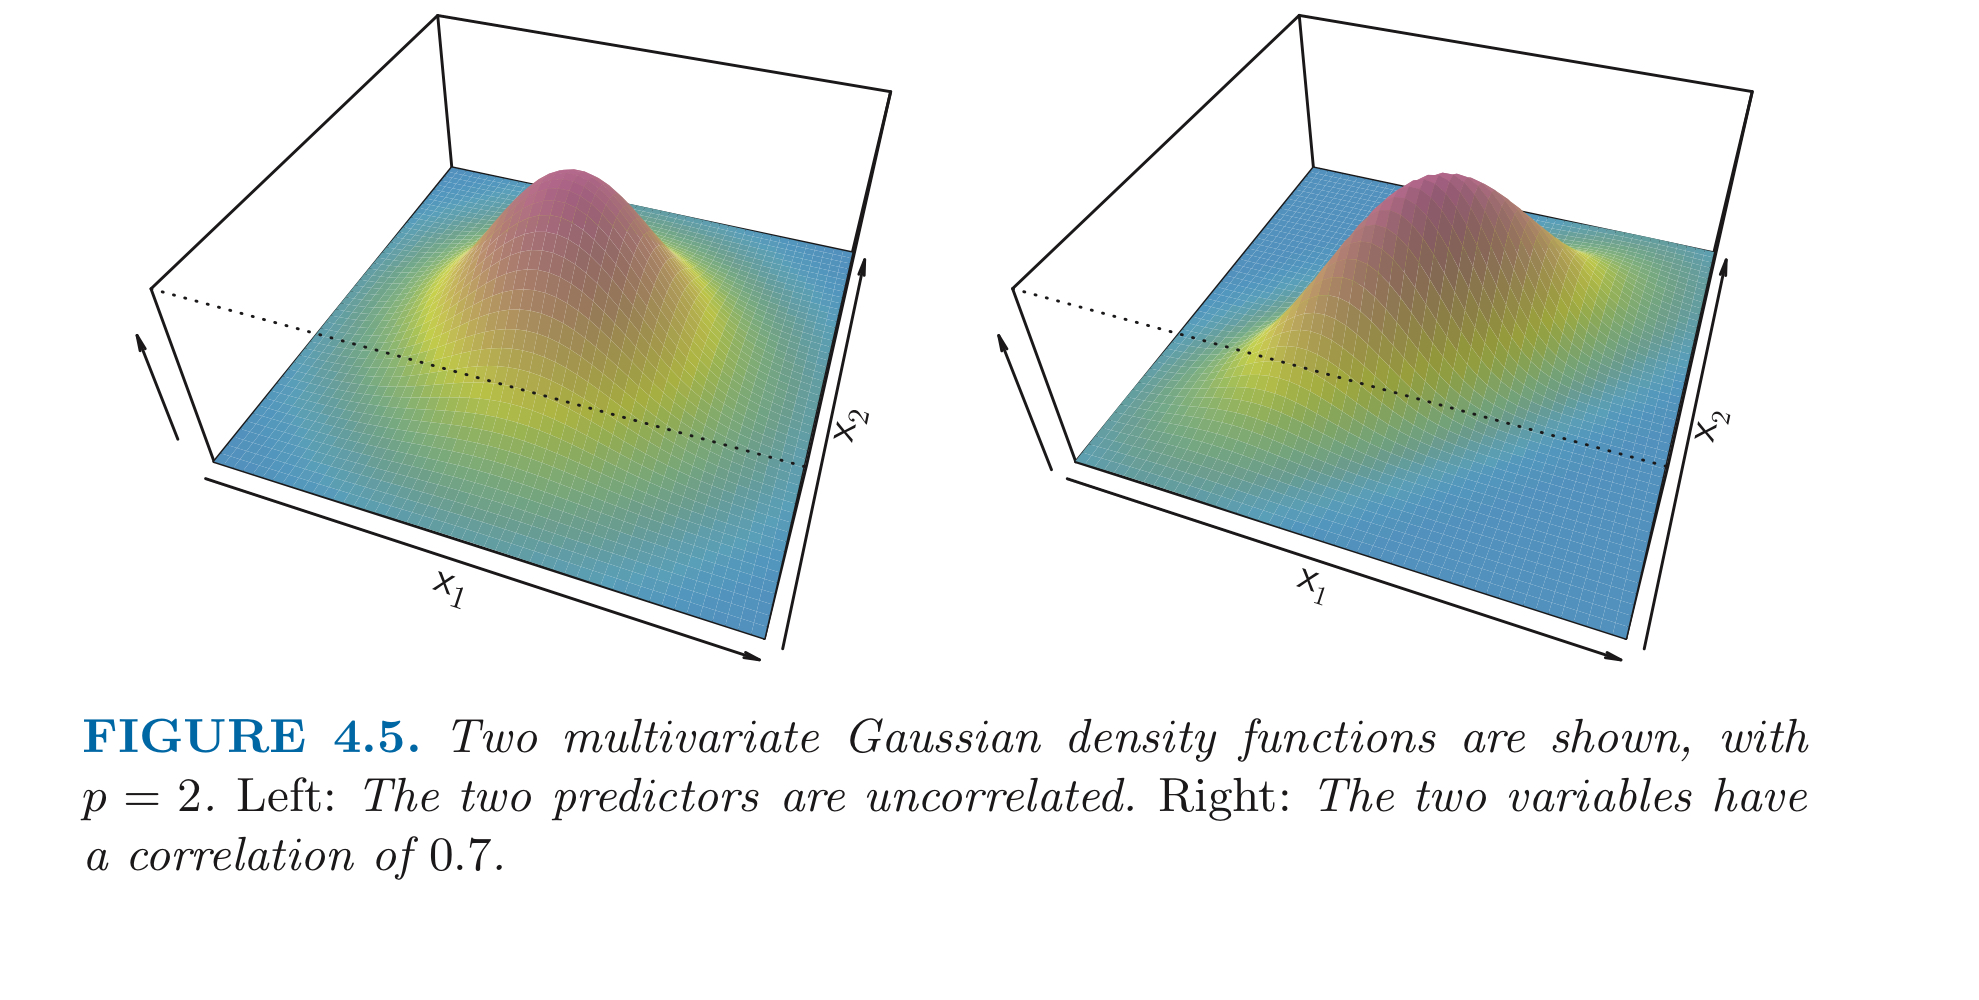
\includegraphics[width=\columnwidth]{MultiVariate Normal.jpeg} % Example image
	\caption{Multivariate Normal Dist}
	\label{multi-normal}
\end{figure}

Think of one dimensional as collapsing into the left side or down. If the var is equal and correlation=0
then the image on the left in \ref{multi-normal} with a circular bottom is produced, if otherwise skewed,
as shown on the right.

\begin{equation}
	X \sim N(\mu,\sum); \mu:\; mean\; vector, \sum:\; covariance\; matrix
\end{equation}

\subsubsection{How is multi preditor LDA used?}

Using the multi variate normal dist values can create the vector/matrix version of the Bayes 
classifier boundary. If there are >2 classes the boundary will be shown as pair of classes.

\subsubsection{Issues to be aware of from multi LDA}

Small distribution between classes in the data set can result in good training error rates, but 
poor test error rates.

\subsection{What is a confusion matrix?}

Determine which type of error is being made in terms of the classes, comparing the error rate for
each class.\\

Sensitivity: Sensitivity is the percentage of true positives (e.g. 90\% sensitivity = 90\% of people who have the target disease will test positive)\\
Specificity: Specificity is the percentage of true negatives (e.g. 90\% specificity = 90\% of people who do not have the target disease will test negative).

\subsection{How to accomdate non equal classes?}

If the bias between classes is not equal the boundary can be altered to instead of being the max,
match the criteria of the problem.

\subsection{What is ROC curve?}

Shows the error rate using different thresholds, the overall peformance of the model is the
area under the curve.\\

If area under the curve is <=0.5 its assumed the performance is no better than chance.

\subsection{Different classification measurments}

\begin{figure}[h] % [h] forces the figure to be output where it is defined in the code (it suppresses floating)
	\centering
	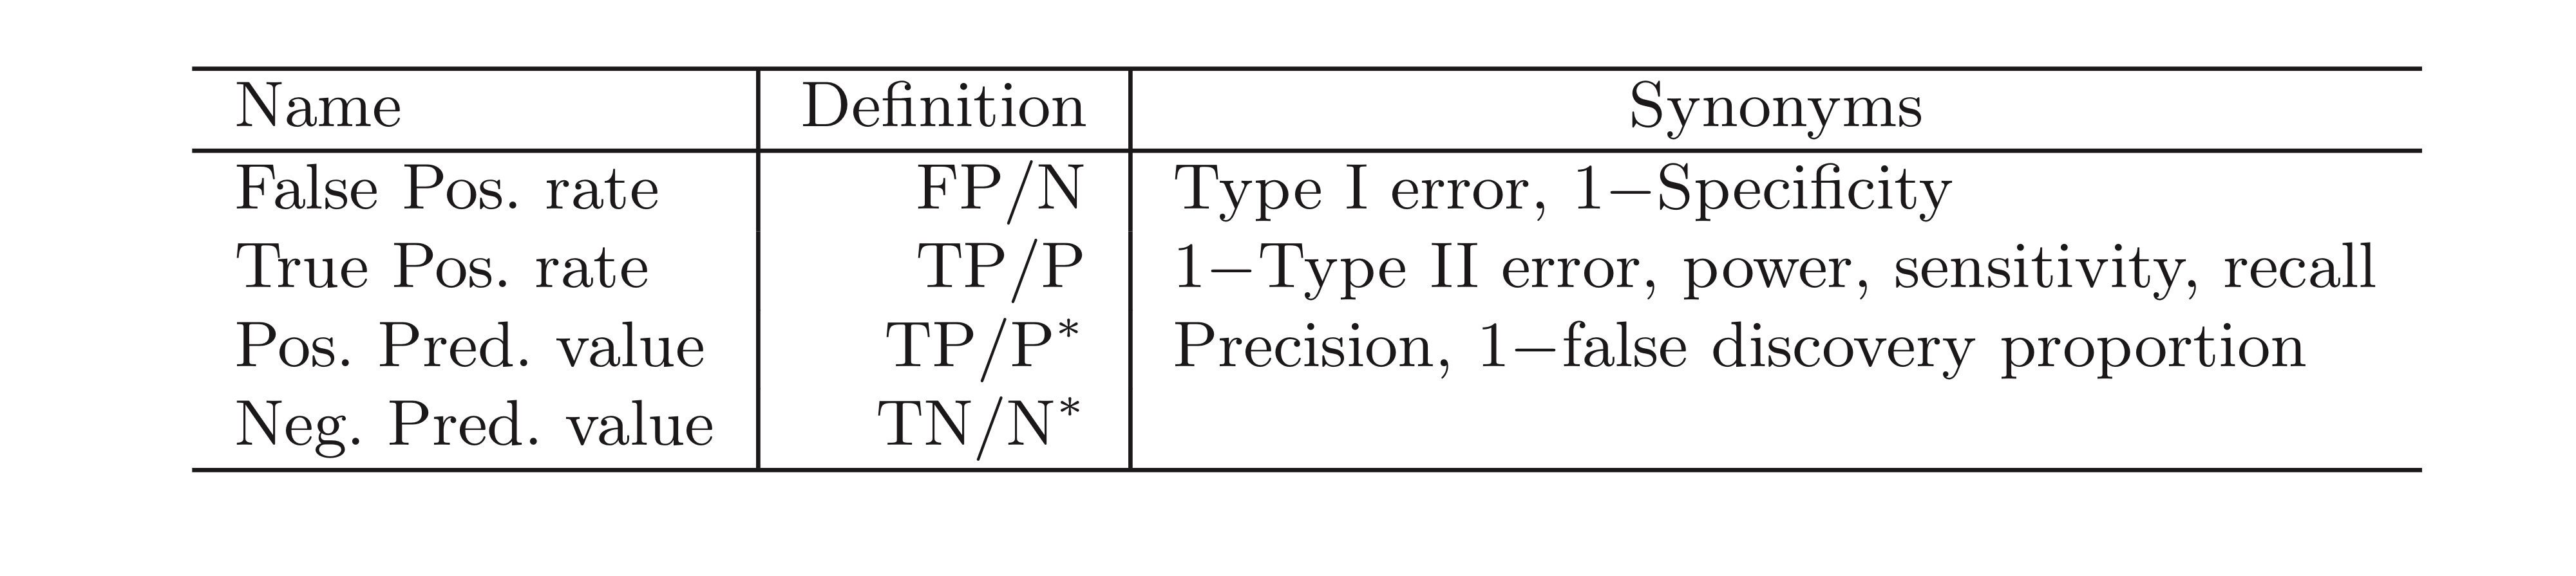
\includegraphics[width=\columnwidth]{classifcation table.jpeg} % Example image
	\caption{Types of classification measurments}
\end{figure}

\subsection{Quadratic Discrimanant Analysis}

The main differnce to LDA is that there is not an assumption of common variance between distribution,
this leads to a quadratic boundary function. 

\subsubsection{What are the pros/cons of QDA?}

More flexiblie, accomdates differing class distributions and therefore has lower bias.\\

It is more compute intensive and has higher variance.

\subsubsection{How do you choose between LDA and QDA?}

Compare the correlation between class and observations for each class, if they are all similar shows
the variance is likley similar. And thefore LDA is a good choice otherwise QDA is.

\subsection{How do you choose between LDA and Logistic for binary scenarios?}

Main differntial is that LDA assumes normal distribution of class, logistic does not.

\subsection{Differences with KNN?}

Descion boundaries cant be weigted towards classes, however it is the most flexible choice.

\subsection{Methods to improve non linear performance?}

Can improve non linear peformance by adding transformed predictors, ie \(X_1^2,X_2^2\) etc.

\section{Resampling methods}

Completley seperate data as the test set may not make sense to use as that could be used as
a valuable method to train the orignial data set. So instead you can repeatadley draw samples
from the data set you have and refit the model and compare to other samples as test data to gain
info about the models setup.\\

\textbf{Model assessment:} Evaluating a models performance.

\textbf{Model selection:} Determining a models flexibilty.\\

\textit{Side note: Can determine if a transformation is valid using hypothesis tests.}

\subsection{Cross Validation}

\subsubsection{What is the validation set approach?}

Randomly divide the data into a training and test set. The issue is there will be less data used
for training the model with each split, will most likley overestimate the test error.

\subsubsection{What is leave one out cross valiation (LOOCV)?}

Use a single observation as the validation set, the rest as training and loop through all data points.

Use the average MSE from all models and validations point:

\begin{equation}
	CV_n = \frac{1}{n} \sum MSE
\end{equation}

The benefits to this are:
\begin{enumerate}
	\item less bias in model as the training set is much bigger
	\item No randomness in method so consistent results produced
\end{enumerate}

This is a very flexible method, however, does require large computation.

\subsubsection{What is K fold cross validation?}

Seperate into K sets, 1 set is the validation and the rest are used for training. Loop through switching
the validation set to each Kth set, taking the average across n sets as the error. 
The main benefit is the computational costs.

Generally the result produced for using K as a reasonable number (>5), produces a result similar to
LOOCV (K=n).\\

The mean of many highly correlated samples has a higher variance than if uncorrelated. And therefore
kCV will produce a low variance than LOOCV but higher bias (less training data used).\\

A good var-bias balance is found around k=5 and k=10, and cleaner to use a multipe of the n as k.
K fold is the main method to compare different models looking for the the bottom of the error over the
different models.

\subsection{Bootstrap}

Bootstrapping involves altering the orginal data set to make estimates on the accuracy of the data.
An example of bootstrapping is randomly duplicating and replacing observations throughout the data set
to get new data to train and validate on. Other types include "Smooth sampling" zero centered (mean) 
adding noise to noraml dist data. \\

This can be applied to a wide range of statistical methods, especially useful for models whos variance
is difficult to measure.

\section{Regularisation}

If the number of predictors is greater than the number of observations, least square method cannot be 
used, it will produce incorrect results.

Irrelevant predictors will lead to unwanted complexity in the model and wasteful computation, the following are methods
to reduce the number of predictors.\\

Methods below normally assume linear regression is being used and therefore RSS is being minimised.

\begin{enumerate}
	\item Subset: Choose a subset of predictors.
	\item Shrinkage (Normalisation): Set some parameters to 0.
	\item Dimension reduction: Project p onto M space.
\end{enumerate}

\subsection{How do you use subsets?}

Compare all possible combination of predictors (\(2^p\)). 
Choose the best in terms of RSS or \(R^2\) for each set number of predictors.
Choose the best overall with AIC, BIC or adjusted \(R^2\).

\subsubsection{How does it work with logistic regression?}

Use deivance instead of RSS, which is the -2* maximum log liklehood.

\begin{equation}
	D_{M} = -2 \log (L_M)
\end{equation}

\(L_M\) : Max achievevale liklehood.

\subsection{How do you pefrom step wise subset ?}

Add one predictor on every iteration, each time trying all possible predictor combination for that
set number of predictors. Then based on the previous best add another predictor. \\

When comparing two models with the same number of predictors can use \(R^2\) or RSS, however differing
predictor number AIC,BIC or adjusted \(R^2\) should be used.

\subsubsection{What is the pros/cons to this method?}

Reduce the iterations to p(1+p)/2. The con is possibly missing different combinations that together
produce a better model than working in the best approach method.\\

To combat this backward stepwise can be used aswell as some hybrid methods that allow better scoping of
possible combinations.

\subsection{How do you compare test error for different models?}

Two methods: Adjust training data to remove bias or use cross validation.\\

How to determine the error parameter to compare:

\begin{itemize}
	\item \(C_p\)
	\item Alkaline Information Criterion (AIC)
	\item Bayesian Information Criterion (BIC)
	\item \(R^2\)
\end{itemize}

\begin{equation}
	C_p = \frac{1}{n}(RSS+2d\sigma^2);\; d:predictors
\end{equation}

This adds a penatlty of 2d var to the RSS error. For least squares AIC is porportinal to Cp.

\begin{equation}
	AIC = \frac{1}{n\sigma^2}(RSS+2d\sigma^2)
\end{equation}

\begin{equation}
	BIC = \frac{1}{n}(RSS + log(n)d\sigma^2)
\end{equation}

BIC provides a larger pentaly for more predictprs as when n>7 log(n) >2.

\begin{equation}
	Adjusted\; R^2 = 1 - \frac{RSS/(n-d-1)}{TSS/(n-1)}
\end{equation}

\begin{equation}
	TSS = \sum{(y_i - \bar{y})^2}
\end{equation}

Balances RSS by increasing the denominator in terms of the number of predictors, ensuring
the number of predictors provides enough benefit in RSS to make it worth it.

\subsection{How does cross validation compare?}

Cross validation does not assume any model form and so is preffered in comparing models.

\subsection{What is the one standard error rule?}

Choose the lowest predictor error score in a cross validation which is within one standard error (of the MSE for each model)
of the lowest CV error.

\section{Shrinkage?}

Reduce the parameters of the model, two methods: Ridge regression and LASSO.

\subsection{Ridge regression}

Adds a penalty to the standard RSS, to push during the minimisation the parameters towards 0.

\begin{equation}
	RSS + \lambda \sum^p_{j=1}{\beta^2_j}
\end{equation}

\(\lambda =0\) : no effect\\
\(\lambda ->\infty \) : Impact grows\\
\(\beta_0 = \bar{y},x_i=0\) 

\subsubsection{How is ridge regression effected by scaling?}

As scaling will directlt effect the penalty value (unlike standard linear regression), therefore
predictors should be standardised to the same unit before applying ridge regression.

\subsubsection{How does the penalty effect bias variance trade off?}

As \(\lambda\) increases the bias will also increase and variance will decrease. However, there
is a balancing point up to which there is not much impact on bias.

\subsubsection{In non linear settings how are vectors compared?}

\(l_2\) (ell-2) is used to compare vectors and is a measured of vector from 0.

\begin{equation}
	||\beta||_2=\sqrt{\sum^p_{j=1}{\beta_j^2}}
\end{equation}

Can be used to compare ridge parameters vs standard LSE parameters.

\subsection{LASSO}

Ridge regression does not set any of the values to 0, instead they tend toward 0. LASSO uses
a slightly different penalty that allows for parameters to become 0, allowing variable selection.

\subsubsection{What is the penalty?}

\begin{equation}
	RSS + \sum{|\beta_j|}
\end{equation}

\subsubsection{How are the regularisation methods shown in a constraint form?}

\textbf{LASSO:}
\begin{equation}
	minimise_{\beta}(RSS)\;\;\;\; subject\; to\; \sum^p_{j=1}{|\beta_j|} \leq s
\end{equation}

\textbf{Ridge Regression:}
\begin{equation}
	minimise_{\beta}(RSS)\;\;\;\; subject\; to\; \sum^p_{j=1}{\beta_j^2} \leq s
\end{equation}

\textbf{Subset:}
\begin{equation}
	minimise_{\beta}(RSS)\;\;\;\; subject\; to\; \sum^p_{j=1}{I(\beta_j\neq 0)} \leq s
\end{equation}

\subsubsection{How does graphing shows the interaction of the constraints?}

\begin{figure}[h] % [h] forces the figure to be output where it is defined in the code (it suppresses floating)
	\centering
	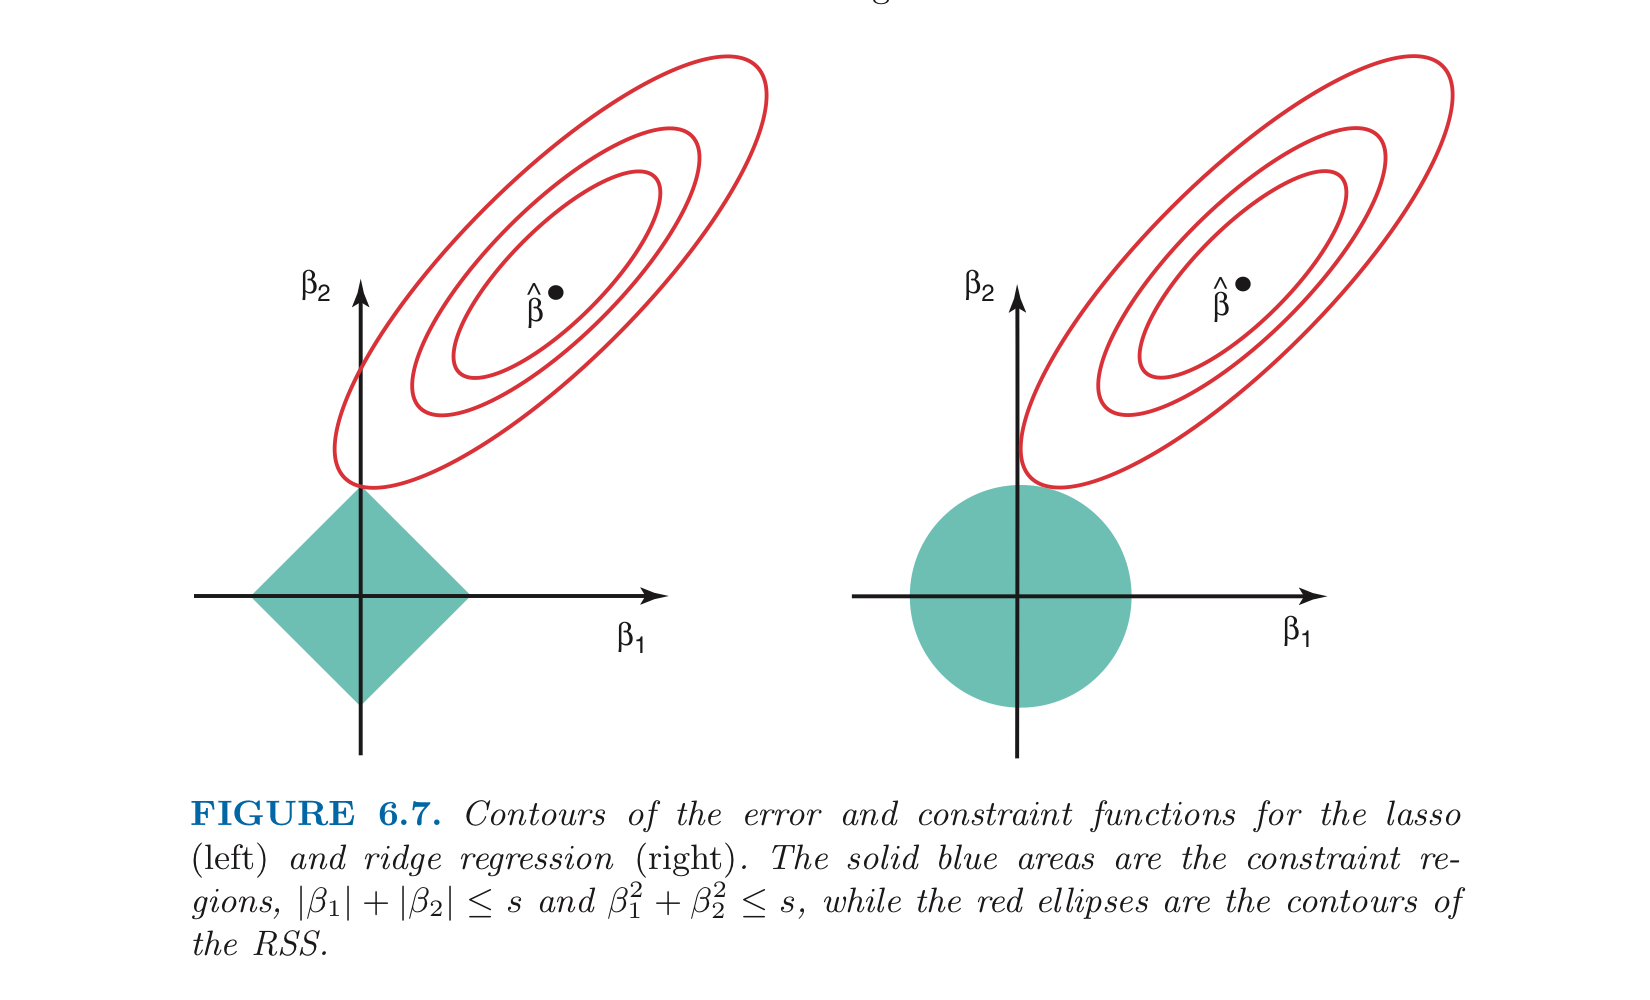
\includegraphics[width=\columnwidth]{ridge vs lasso.jpeg} % Example image
	\caption{ridge vs lasso; p=2, elipses are constant RSS vals}
\end{figure}

\subsubsection{How does ridge compare to lasso?}

Ridge should be used if all predictors truly relate to the outcome, otherwise lasso is the best bet.\\

Cross validation should be used to calculate the best lambda and compare ridge and lasso solutions.

\subsection{Dimension reduction?}

Projection of p predictors to M where M<p:\\

Below are the vectors Z which is X predictors linearly combined to create M predictors.
\begin{equation}
	Z_m = \sum^p_{j=1}{\phi_{jm}X_j}
\end{equation}

Theta combined with phi for M results in the beta parameters. Giving a smaller M parameters, due to this
mapping all M paramters are combined with a specific phi set of values to give the orginal parameter.
\begin{equation}
	y_i= \theta_0 + \sum^M_{m=1}{\theta_mz_{im}}
\end{equation}
\begin{equation}
	\beta_j = \sum^M_{m=1}{\phi_{jm}\theta_m}
\end{equation}

Reducing the dimensions will reduce the variance, and can avoid overfitting as it is a concentration
of the data.

\subsubsection{What is principal component analysis?}

The first principle component is the line which if the points were projected onto would give the
most variance (ie distance from points to line). To confine this we use the contraint 
\(\phi_{11}^2 + \phi_{21}^2 =1; (\phi_{jm})\).\\

The second principal has max variance but is also uncorrelated to the first pc, and therefore will
be perpindicular to it.

\subsubsection{What is principal components regression approach?}

Determine the first M Z principal components and uses them as predictors for a regression line.
The idea is that most of the relationship with the response is in the first few principal components.\\

Or the direction in which the observations show the most variation is directions assocaited with the response,
which is what the principle components are.\\

If this is true dimension reduction will produce a less overfit model which peforms better. Reccomended
to standardise the variables onto the same scale, as it will effect the variance between predictors.

\subsection{What to do in high dimensional problems (p>>n)?}

Things to be aware of:

\begin{itemize}
	\item Dimnesional model comparison isnt effective (AIC,BIC,\(R^2\))
	\item Careful of collinearity, where removing predictors is difficult due to thier linear relationship.
\end{itemize}

\section{Non linear regression}

5 main methods:

\begin{enumerate}
	\item \textbf{Polynomial regression:} Add extra predictors by raising each by a power
	\item \textbf{Step functions:} Split the range of a variable into sections making it a classification problem
	\item \textbf{Regression splines:} Divide into sections, fit a polynomial that is constrained to be smooth
	at the boundary.
	\item \textbf{Smoothing splines:} Use residual sum of squares subject to a smoothness penalty similar to regression splines.
	\item \textbf{Local regression:} Allows splines to overlap at the boundaries in a smooth way.
	\item \textbf{Generalised additive models:} Extend methods to deal with more predictors.
\end{enumerate}

\subsection{Generalised additive Models}

Create additive non linear model for p predictors.\\

For regression:

\begin{equation}
	y = \beta_0 + x_{i1}\beta_1 + x_{i2}\beta_2
\end{equation}

Can be transformed to:

\begin{equation}
	y = \beta_0 + f(x_{i1}) + f(x_{i2})
\end{equation}

In which each function is its own model for that predictor.\\

For classifcation:

\begin{equation}
	log\frac{p(x)}{1-p(x)} = \beta_0 + f(x_{i1}) ... + f(x_{ip})
\end{equation}

\subsubsection{What is backfitting?}

For some methods its not as simple as adding the models, in which case backfitting is used.
Combines models by updating the fit for each predictor in turn keeping the others fixed.

\subsubsection{What is the con of GAMs?}

As it is additive the interaction between predictors can be lost, but can mitigate this by adding
combined function predictors ie f(\(x_{i1},x_{i2}\)).

\section{Tree based methods}

The idea behind tree based methods is to segement the observations, with rules that can be summerised
as a tree. \\

Simple tree methods dont compare well in terms of accuracy to other modelling methods, however, are easy
to visualise and use for inference.\\

To improve predictive performance can use multiple tree together; bagging, random forests and boosting
are examples of this.

\subsection{How do trees work?}

Splitting the observations into sections based on the predictor values, this can be done by stepping
through each predictor.

\begin{figure}[h] % [h] forces the figure to be output where it is defined in the code (it suppresses floating)
	\centering
	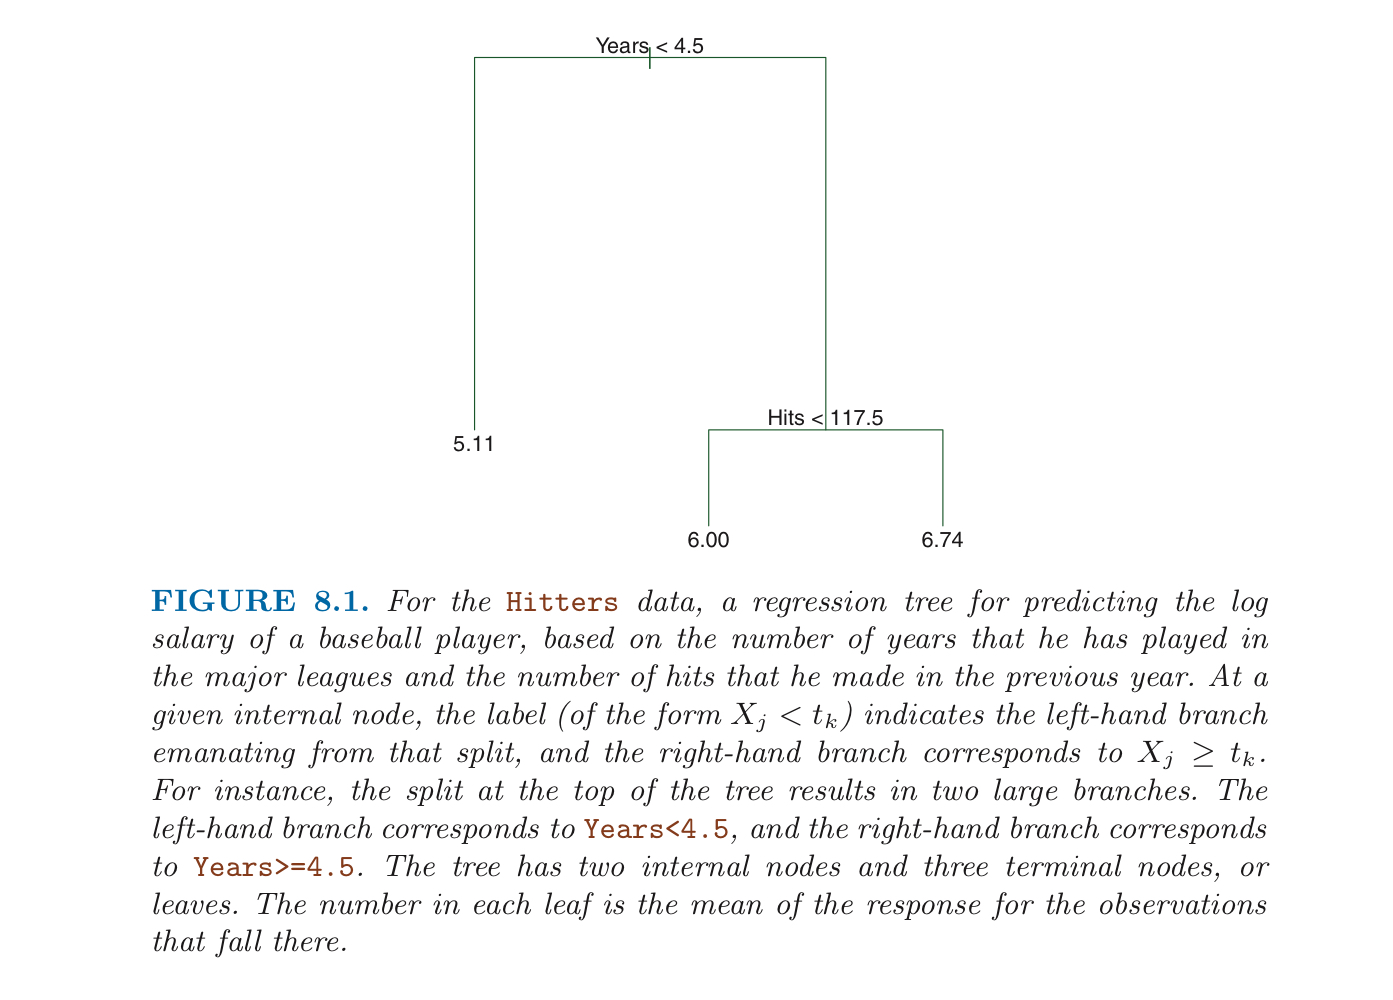
\includegraphics[width=\columnwidth]{Tree example.jpeg} % Example image
	\caption{Tree split example}
\end{figure}

The mean in each section is often used as the default response, if the observation lies in that section.
It can also be used for inference.

\subsection{How to determine the regions?}

A possible method is minimising the RSS from the mean value of each region:

\begin{equation}
	\sum^J_{j=1}\sum_{i\epsilon R_j}{(y_i-\hat{y}_{Rj})}^2
\end{equation}

J: is the region.\\
\(\hat{y}_{R_j}\): is the mean of the region.

\subsection{What is top down greedy approach recursive binary splitting?}

Working from the top of the tree splitting into two for each predictor, greedy as it does not
look ahead only works step by step. Until a stopping criterion is reached ie each region will have
n>5. This could lead to overfitting of the tree.

\subsection{When should the splitting stop?}

An alternative is to split until the a chosen RSS value. But a better method is to let the full 
tree be created and then work through the tree subsets comparing each other in terms of error rate.

\subsection{How can you limit the number of subsets compared?}

\textbf{Pruning} allows a selection of the subset via penaltys added to the minimisation:

\begin{equation}
	\sum^{|T|}_{m=1}\sum_{i\epsilon R_m}{(y_i-\hat{y}_{Rm})}^2 + \alpha|T| 
\end{equation}

T: Number of terminal nodes on the tree.\\

Similar to LASSO this will allowing reduce the number of terminal nodes, alpha is chosen via cross
validation.

\subsection{How is it used with Classification?}

Use the most commonly occuring class in the region as the default response. And use error rate
instead of RSS to choose regions.

\begin{equation}
	E = 1-max_k(\hat{p}_{mk})
\end{equation}

\(\hat{p}_{mk}\): Portion of training observations in the mth region that from the kth class.

\subsubsection{Alternatives to using error rate?}

Error rate can be not sensitive enough so Gini Index is used:

\begin{equation}
	G = \sum^k_1{\hat{p}_{mk}(1-\hat{p}_{mk})}
\end{equation}

Gini index will take a small value if the p value is close to 0 or 1 and therefore kind of shows
node purity in that the when the porportion of the class is very low or high Gini is low.

Can also use cross entropy function which is similar.

\subsection{What are pros/cons?}

Pros:
\begin{itemize}
	\item Easy to explain
	\item Easy to display
	\item Easily handles qualitative (easy dummy values as a split)
\end{itemize}

Cons:
\begin{itemize}
	\item Poor predictive accuracy
\end{itemize}

If the relationship is highly non linear and complex trees maybe the preffered model.

\subsection{What is bagging?}

Bootstrapping or bagging reduces the variance of a model, combining the averages of observations sets
will give a lower variance than each set.

So using bootstrapped models and aggregating them will achieve a lower variance.

\subsubsection{What is out of bag?}

If during the bootstrap a model uses 2/3 of the observations, the other 1/3 is OOB. This is used
as the test set and if any other model has the same OOB the error is aggregated.

This can be used with subset selection methods to get better trees to combine via bootstrapping.

\subsection{What are Random forests?}

The trees are decorrelated and combined just as in bagging. Ensuring the trees when combined have a
mixed structure is done by randomly selecting a sample of m predictors to build the tree. m is often
the square root of p.

\subsection{What is Boosting?}

Similar to bagging but sequential. Calculate tree, add factor of tree to overall function, take away
response from that model from the residuals (shown below):

Fraction addition of model, where r the residuals are used as the response:
\begin{equation}
	\hat{f}(x) += \lambda \hat{f}^b(x)
\end{equation}

Update the residuals:
\begin{equation}
	r_i -= \lambda \hat{f}^b(x_i)
\end{equation}

Final model:
\begin{equation}
	\hat{f}(x) = \sum^B_{b=1}{\lambda\hat{f}^b(x)}
\end{equation}

\(\lambda\): Shrinkage parameter, controls the speed of learning.\\
B: number of tree models created.\\

Due to the learning process increasing B does not cause overfitting.

\section{Support Vector Machines}

One of the best out of the box classifiers, intended for binary class cases.

\subsection{What is the hyperplane?}

In p dimensional space, plane is p-1 subspace. Ie in 3 dimensional space the plane is flat.

\begin{equation}
	\beta_0 + \beta_1X_1 + \beta_2X_2 + \cdots \beta_pX_p = 0
\end{equation}

\begin{equation}
	X = (X_1,X_2,\cdots X_p)^T
\end{equation}

A point that satisfies the above two equation lies on the hyperplane. The hyperplane cuts the space
in half about 0, can determine on which side of the hyperplane the point is by using the equation.\\

Also shows the certainty of the response based on the distance from the hyperplane boundary.

\subsection{What is the maximal margin classifier?}

The minimum perpendicular distance from all observations to the plane (the margin), is maximised. Support vectors
are the points that the hyperplane relies on and used to determine the margin (the closest points).

\begin{equation}
	y_i(\beta_0+\beta_1x_{i1}+\beta_2x_{i2}+\cdots \beta_px_{ip}) \geq M
\end{equation}

M: Instead of being 0, adds a cushion for the decision boundary, this is also the margin.\\

The margin (perp distance to hyperplane) is given by:

\begin{equation}
	y_i(\beta_0+\beta_1x_{i1}+\beta_2x_{i2}+\cdots \beta_px_{ip})
\end{equation}

\subsection{What if there is no perfect hyperplane?}

In many cases cannot maximise M>0, as there is no hyperplane perfectly separating the two.
In this case a soft margin is used, which almost completely separates the observations, this
is called the \textbf{support vector classifier}.\\

Furthermore, in many cases even if there exists a perfect solution the variance will be very high
as a single observation could change the hyperplane.

\subsection{What is the support vector classifier?}

Maximise M:

\begin{equation}
	y_i(\beta_0+\beta_1x_{i1}+\beta_2x_{i2}+\cdots \beta_px_{ip}) \geq M(1-\epsilon_i)
\end{equation}

\begin{equation}
	\epsilon_i \geq 0,\; \sum \epsilon_i \leq C
\end{equation}

C: Non negative tuning parameter\\
\(\epsilon\): Slack variable \\

This allows the support vectors to have a distance less than the margin, depending on epsilon and
C. If \(\epsilon>0\) the point is on the wrong side of the margin if \(\epsilon>1\) its on the wrong
side of the hyperplane. C determines the severity of the violations, controlling the bias-var
trade off and is chosen via cross validation.\\

\textbf{Support vector classifiers are not effected by outliers!}

\subsection{How do you make the plane non linear?}

Could use added predictor polynomials to make it non linear but instead the general method is to
use kernals in the support vector machine.

\subsection{What is the support vector machine?}

Focusing on only the support vectors (S) and using inner products (which is used to solve the
support vector classifier) gives the classifier as:

\begin{equation}
	f(x) = \beta_0 + \sum_{i\epsilon S}{\alpha_i\sum^p_{j=1}{x_{ij}x_{i'j}}}
\end{equation}

Can then generalise the inner product of points to be function (kernal):

\begin{equation}
	K\{x_i,x_{i'}\}
\end{equation}

Linear kernal version:
\begin{equation}
	K : \sum{x_ix_{i'}}
\end{equation}

Polynomial kernal version:
\begin{equation}
	K: (1+ \sum{x_ix_{i'}})^d;\; d:Dimensions
\end{equation}

Other kernal options exist ie, radial kernal.

\textbf{Use ROC curve to compare SVM and LDA.}

\subsection{What if the number of classes is >2?}

Use one versus one classifcation, create pairs of classes for all possible combinations and run
all SVMs choosing the highest shown class.\\

One versus all classifcation, one class vs the rest to check with certainty if the observation belongs
to the chosen class.

\subsection{Show SVC in loss penalty form}

Fitting the support vector classifier \(f(x_i) = (\beta_0+\beta_1x_{i1}+\beta_2x_{i2}+\cdots \beta_px_{ip})\):
\begin{equation}
	minimise({\sum^n_{i=1}{max(0,1-y_if(x_i))+\lambda\sum^p_{j=1}{\beta^2_j}}})
\end{equation}

\(\lambda\) acts like C as the penalty term. Can directly compare this form to other methods, which are
made of loss functions and penalty terms, known as hinge loss.

\subsection{How does logitisic and SVM compare?}

If the classifiers are clearly seperated SVM is preffered, in overlapping regions logitisic regression is good.\\

Can also use kernal methods in other classifiers.

\subsection{What about Support vector regression?}

The margin is setup so that absoulte values greater than a constant contribute to the loss to determine
the parameters.\\

\textbf{TODO: ADD MORE INFO}
%----------------------------------------------------------------------------------------
%	FIGURE EXAMPLE
%----------------------------------------------------------------------------------------

% \begin{figure}[h] % [h] forces the figure to be output where it is defined in the code (it suppresses floating)
% 	\centering
% 	\includegraphics[width=0.5\columnwidth]{IMAGE_NAME.jpg} % Example image
% 	\caption{European swallow.}
% \end{figure}

%----------------------------------------------------------------------------------------
% MATH EXAMPLES
%----------------------------------------------------------------------------------------

% \begin{align} 
% 	\label{eq:bayes}
% 	\begin{split}
% 		P(A|B) = \frac{P(B|A)P(A)}{P(B)}
% 	\end{split}					
% \end{align}

%----------------------------------------------------------------------------------------
%	LIST EXAMPLES
%----------------------------------------------------------------------------------------

% \begin{itemize}
% 	\item First item in a list 
% 		\begin{itemize}
% 		\item First item in a list 
% 			\begin{itemize}
% 			\item First item in a list 
% 			\item Second item in a list 
% 			\end{itemize}
% 		\item Second item in a list 
% 		\end{itemize}
% 	\item Second item in a list 
% \end{itemize}

%------------------------------------------------

% \subsection{Numbered List}

% \begin{enumerate}
% 	\item First item in a list 
% 	\item Second item in a list 
% 	\item Third item in a list
% \end{enumerate}

%----------------------------------------------------------------------------------------
%	TABLE EXAMPLE
%----------------------------------------------------------------------------------------

% \section{Interpreting a Table}

% \begin{table}[h] % [h] forces the table to be output where it is defined in the code (it suppresses floating)
% 	\centering % Centre the table
% 	\begin{tabular}{l l l}
% 		\toprule
% 		\textit{Per 50g} & \textbf{Pork} & \textbf{Soy} \\
% 		\midrule
% 		Energy & 760kJ & 538kJ\\
% 		Protein & 7.0g & 9.3g\\
% 		\bottomrule
% 	\end{tabular}
% 	\caption{Sausage nutrition.}
% \end{table}

%----------------------------------------------------------------------------------------
%	CODE LISTING EXAMPLE
%----------------------------------------------------------------------------------------

% \begin{lstlisting}[
% 	caption= Macro definition, % Caption above the listing
% 	language=python, % Use Julia functions/syntax highlighting
% 	frame=single, % Frame around the code listing
% 	showstringspaces=false, % Don't put marks in string spaces
% 	numbers=left, % Line numbers on left
% 	numberstyle=\large, % Line numbers styling
% 	]

% 	CODE

% \end{lstlisting}

%----------------------------------------------------------------------------------------
%	CODE LISTING FILE EXAMPLE
%----------------------------------------------------------------------------------------

% \lstinputlisting[
% 	caption=Luftballons Perl Script., % Caption above the listing
% 	label=lst:luftballons, % Label for referencing this listing
% 	language=Perl, % Use Perl functions/syntax highlighting
% 	frame=single, % Frame around the code listing
% 	showstringspaces=false, % Don't put marks in string spaces
% 	numbers=left, % Line numbers on left
% 	numberstyle=\tiny, % Line numbers styling
% 	]{luftballons.pl}

%------------------------------------------------

\end{document}